\PassOptionsToPackage{sols}{handout}
\documentclass[main]{subfiles}
\setcounterrefbeforedot{chapter}{m-ws3-6}
\setcounterrefafterdot{section}{m-ws3-6}
\addtocounter{section}{-1}
\usepackage{solutions}

\begin{document}

\ifSubfilesClassLoaded{%
  \chaptermark{\chapterthree}
}{}

\section{Problem Solving and Transition to Limits} \label{ws3-6}

\begin{problemonly}
    \begin{framed}

\textbf{Key Ideas}:

\begin{itemize}[topsep=0pt,partopsep=0pt,parsep=8pt,itemsep=0pt]

\item You should be able to use trig and inverse trig functions to solve optimization and related rates problems

\item You should recall how to evaluate limits both algebraically and graphically.

\end{itemize}
\end{framed}
\end{problemonly}

\begin{enumerate}

\item 
\textit{Warm-Up:} In this problem, you'll graph $f(x) = \cos(\arccos x)$.
  \begin{enumerate}
  \item
    \begin{problem}[0.25in]
      What is the domain of $f$?
    \end{problem}

    \begin{solution}
      In order for $f(x)$ to be defined, we first need $\arccos x$ to be
      defined, which means $x$ must be in $[-1, 1]$.  If $\arccos x$ is
      defined, then $\cos(\arccos x)$ will also be defined, so the
      \fbox{domain of $f$ is $[-1, 1]$}.
    \end{solution}

  \item
    \begin{problem}[1in]
      For what values of $x$ is it true that $f(x) = x$?
    \end{problem}

    \begin{solution}
      $f(x)$ is only defined for $x$ in $[-1, 1]$.  If $x$ is any number
      in $[-1, 1]$, let $\theta = \arccos x$.  In words, $\theta$ is the
      angle in $[0, \pi]$ whose cosine is $x$ (that is, $\cos \theta =
      x$).  Then, \[f(x) = \cos \Big( \underbrace{\arccos x}_\theta \Big)
      = \cos \theta = x.\] So, \fbox{$f(x) = x$ for all $x$ in $[-1, 1]$}.
    \end{solution}

  \item
    \begin{problem}[\vfill]
      Compute $f'(x)$ by using the Chain Rule on $f(x) = \cos(\arccos x)$. Simplify completely. (You should get a constant. 
      Why does this make sense?)
    \end{problem}

    \begin{solution}
        We use the Chain Rule:
        \begin{align*}
        f'(x) &= \frac{d}{dx} \left[\cos(\arccos x) \right]\\
        &= -\sin(\arccos x) \cdot \frac{-1}{\sqrt{1-x^2}}
        \end{align*}
        To determine the value of $-\sin(\arccos x)$, we can picture it
        graphically. Let's say $y=\arccos x$. Then $\cos(y)=x=\frac{x}{1}=\frac{\text{adj.}}{\text{hyp.}}$.
    \begin{center}
      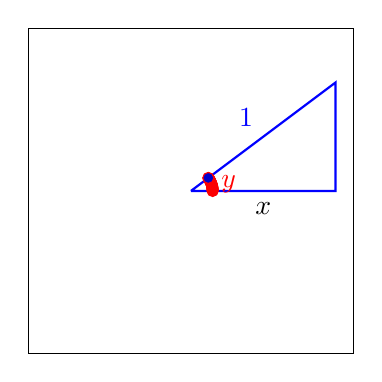
\begin{tikzpicture}
        \begin{axis}[axis equal=true, xmin=-4.5, xmax=4.5, ymin=-4.5,
          ymax=4.5, xtick=\empty, ytick=\empty, width=2.25in,
          height=2.25in, clip=false] %
          \draw[blue, thick] (0,0) --  (4,0) --
           (4,3) -- node[anchor=south east]
          {$1$} (0,0); 
          \node[] at (2,-0.5) {$x$};
          \pgfmathsetmacro{\angle}{atan(3/4)} %
          \addplot+[domain=0:\angle, red, thin, ->, >=to] ({0.6 *
            cos(x)}, {0.6 * sin(x)}) node[pos=0.5, right] {$y$};
        \end{axis}
      \end{tikzpicture}        
    \end{center}
    By the Pythagorean theorem, the missing side of the right triangle is $\sqrt{1-x^2}$. Thus, $\sin y = \sqrt{1-x^2}$. This means that
    \[f'(x)=-\sin(\arccos x) \cdot \frac{-1}{\sqrt{1-x^2}}=\boxed{1}\]
    
        This makes sense because $f(x)=x$ on the entire domain $[0,1]$.
    \end{solution}

  \item

    \note{This is a good opportunity to get them to think about
      consistency.} 

    \begin{problem}[\vfill]
      Sketch the graph of $f$.  Clearly indicate the domain and range.
    \end{problem}

    \begin{solution}
      This is just a matter of putting the previous parts together.  We've
      seen that the domain of $f$ is $[-1, 1]$, and $f(x) = x$ for all $x$
      in $[-1, 1]$.  This tells us the graph of $f$:
      \begin{center}
        \begin{tikzpicture}
          \begin{axis}[xmin=-1.2, xmax=1.2, axis equal=true, width=2in,
            height=2in] 
            \addplot+[scatter, scatter src=explicit symbolic] coordinates
            {
              (1, 1) [closed]
              (-1, -1) [closed]
            };
          \end{axis}
        \end{tikzpicture}
      \end{center}      
    \end{solution}

  \end{enumerate}


\spaceonly{\probonly{\newpage}}
  



\item 
  \begin{problem}[\newpage]
      Find the area of the largest rectangle that can be inscribed in a
      semicircle of radius $2$.

    \begin{center}
      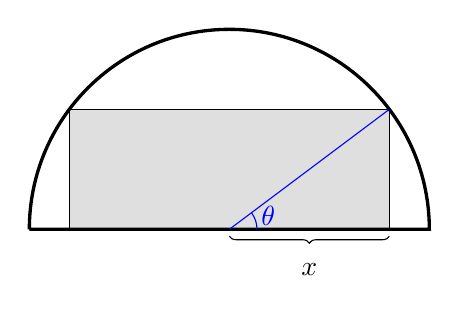
\begin{tikzpicture}[x=1in, y=1in]
        \draw[fill=lightgray!50!white] (-0.8, 0) -- (-0.8, 0.6) -- (0.8, 0.6) -- (0.8, 0) -- cycle;
        \draw[very thick] (-1, 0) -- (1, 0) arc[radius=1, start angle=0,
        end angle=180];
        \draw[blue] (0, 0) -- (0.8, 0.6);
        \draw[blue] (10pt, 0) arc[radius=10pt, start angle=0, end
        angle=atan(3/4)] node[right, yshift=-1pt] {$\theta$}; 
        \draw[decorate, decoration={brace, mirror}, yshift=-.25em] (0,0) -- (0.8,0);
        \node[] at (0.4,-0.2) {$x$};
      \end{tikzpicture}
    \end{center}

    There are actually two different ways of solving this problem: expressing the area of the rectangle in terms of the length $x$, OR expressing the area of the rectangle in terms of trigonometric functions and the angle $\theta$. Both methods should give the same maximum area! 
  \end{problem}

  \begin{solution}
    This is an optimization problem because we're trying to make something
    as large as possible. 

    \highlight{\textbf{Goal:} Maximize area of rectangle.}

    \ideas{Next, we write a formula for the thing we're trying to maximize
      (area of the rectangle); we're asked to do this in terms of $\theta$.}

    To start, we know that the area of the rectangle (let's call that $A$)
    is $\text{width} \cdot \text{height}$.  We can express the width and
    height in terms of $\theta$ using the blue right triangle:
    \begin{center}
      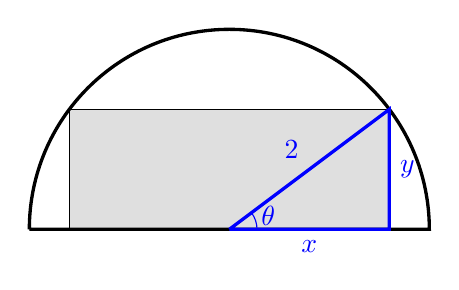
\begin{tikzpicture}[x=1in, y=1in]
        \draw[fill=lightgray!50!white] (-0.8, 0) -- (-0.8, 0.6) -- (0.8,
        0.6) -- (0.8, 0) -- cycle; %
        \draw[very thick] (-1, 0) -- (1, 0) arc[radius=1, start angle=0,
        end angle=180]; %
        \draw[blue, very thick] (0, 0) -- node[anchor=south east]{$2$}
        (0.8, 0.6) -- node[right] {$y$} (0.8, 0) -- node[below]{$x$} (0,
        0); %
        \draw[blue] (10pt, 0) arc[radius=10pt, start angle=0, end
        angle=atan(3/4)] node[right, yshift=-1pt] {$\theta$};
      \end{tikzpicture}
    \end{center}
    (The triangle has hypotenuse 2 because that's the radius of the
    semicircle.)  From the right triangle, we see that $\sin \theta =
    \frac{y}{2}$ and $\cos \theta = \frac{x}{2}$, so $y = 2 \sin \theta$
    and $x = 2 \cos \theta$.  The rectangle has width $2x = 4 \cos \theta$
    and height $y = 2 \sin \theta$, so its area in terms of $\theta$ is
    \[ A(\theta) = (4 \cos \theta)(2 \sin \theta) = 8 \sin \theta \cos
    \theta.\] \ideas{Now, maximize!} First, since we're thinking of
    $\theta$ as an angle in a right triangle, we're only interested in
    what happens when it's between $0$ and $\frac{\pi}{2}$.  So, we're
    trying to maximize $A(\theta)$ on $\left[0, \frac{\pi}{2}
    \right]$.\footnote{You might argue that the domain should instead be
      $\left( 0, \frac{\pi}{2} \right)$, since $\theta$ can't actually be
      $0$ or $\frac{\pi}{2}$.  This is true, but we often include the
      endpoints in our interval when we optimize just because it may be
      easier to optimize on a closed interval.  If something goes wrong
      when we optimize on the closed interval -- for example, the function
      ends up undefined at one of the ``fake'' endpoints -- then we have
      to go back and look more closely at what happens on the open
      interval.}  We want the critical points, so we should first find
    $A'(\theta)$.  By the Product Rule, $A'(\theta) = 8 (\cos^2 \theta -
    \sin^2 \theta)$.  This is never undefined; let's figure out where it
    is 0 on $\left[ 0, \frac{\pi}{2} \right]$.  In order to have
    $A'(\theta) = 0$, we must have
    \begin{align*}
      \sin^2 \theta &= \cos^2 \theta \\
      \frac{\sin^2 \theta}{\cos^2 \theta} &= 1 \\
      \tan \theta &= \pm 1
    \end{align*}
    The only solution of $\tan \theta = \pm 1$ in $\left[ 0, \frac{\pi}{2}
    \right]$ is $\theta = \frac{\pi}{4}$.  So, the critical points of
    $A(\theta)$ on $\left[ 0, \frac{\pi}{2} \right]$ are $0,
    \frac{\pi}{4}, \frac{\pi}{2}$.  (Remember that endpoints of a closed
    interval are always considered critical points.)  Since we're working
    on a closed interval, an easy way to find the absolute maximum is just
    to evaluate our function at all of the critical points and see which
    gives the highest value:
    \begin{align*}
      A(0) &= 8 \sin 0 \cos 0 = 0 \\
      A \left( \frac{\pi}{4} \right) &= 8 \sin \frac{\pi}{4} \cos
      \frac{\pi}{4} = 4 \\
      A \left( \frac{\pi}{2} \right) &= 8 \sin \frac{\pi}{2} \cos
      \frac{\pi}{2} = 0
    \end{align*}
    So, the maximum area is $\boxed{4}$.

    \emph{Note:} If you said the domain was $\left(0, \frac{\pi}{2}
    \right)$, then you'd have just one critical point, $\theta =
    \frac{\pi}{4}$, and you could use the First Derivative Test or Second
    Derivative Test to see that this is the absolute maximum.
  \end{solution}

\item  % Andrew Dittmer

  \emph{For homework, you derived the \textbf{Law of
      Cosines}, which says that if we have a triangle with sides of length
    $a$, $b$, and $c$ and if $\theta$ is the angle opposite the side of
    length $c$, then $c^2 = a^2 - 2ab \cos \theta + b^2$.  That will be
    useful in the following problem.}

  \begin{problem}[\newpage]
    A slingshot is made out of two sticks, one of length $2$ inches and
    one of length $4$ inches.  The two sticks are tied together at one
    end.  The other end of the two sticks is connected by a rubber band.
    Someone is flexing the angle of the two sticks.  When the angle
    between the two sticks is $60^{\circ}$, the angle is increasing at a
    rate of $10^\circ$ per second.  How quickly is the length of the
    rubber band increasing?
  \end{problem}

  \begin{solution}
    \ideas{As usual, let's start by drawing two pictures, a generic
      picture that applies at any time, and a ``snapshot'' showing the
      situation at the time we care about.  We'll also label some
      variables in the generic picture.}  In the pictures below, the
    rubber band is the dashed line.

    \begin{center}
      \begin{tabular}{ccc}
        \emph{Snapshot} & \hspace{0.25in} & \emph{Generic} \\
        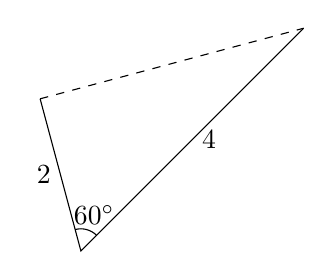
\begin{tikzpicture}
          \coordinate (A) at (105:2); %
          \coordinate (B) at (45:4); %
          \draw (A) -- node[left]{2} (0, 0) -- node[right] {4} (B); %
          \draw[dashed] (A) -- (B); %
          \draw (45:8pt) arc[radius=8pt, start angle=45, end angle=105]; %
          \draw (70:14pt) node{$60^\circ$}; %
        \end{tikzpicture} &&
        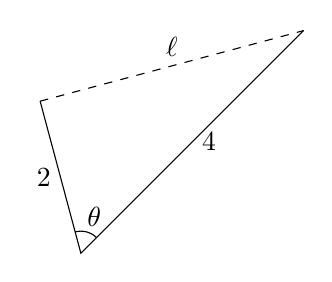
\begin{tikzpicture}
          \coordinate (A) at (105:2); %
          \coordinate (B) at (45:4); %
          \draw (A) -- node[left]{2} (0, 0) -- node[right] {4} (B); %
          \draw[dashed] (A) -- node[above]{$\ell$} (B); %
          \draw (45:8pt) arc[radius=8pt, start angle=45, end angle=105]; %
          \draw (70:14pt) node{$\theta$}; %
        \end{tikzpicture}        
      \end{tabular}
    \end{center}

    \ideas{Next, we figure out what we know and what we want to know.}

    \highlight{ \textbf{What we know:} $\frac{d\theta}{dt}$ is 10 degrees
      per second, but we always want to work in
      radians,\footnotemark\, so $\frac{d\theta}{dt} =
      \frac{\pi}{18}$ radians per second

      \textbf{What we want to know:} $\frac{d\ell}{dt}$
    }    
    \footnotetext{The reason we want to use radians is that the
        derivatives of trig functions we found are only true if we work in
        radians; you looked at this issue in
        {{{Problem Set 13}, {{\#5}}}}.}

    \ideas{Now, we try to relate variables.  In this case, since the rates
      we know is $\frac{d\bm{\theta}}{dt}$ and the rate we want to know is
      $\frac{d\bm{\ell}}{dt}$, we try to relate $\theta$ and $\ell$.}  By
    the Law of Cosines, we get:

    \highlight{\textbf{Equation relating our variables:} $\ell^2 = 2^2 - 2
      \cdot 2 \cdot 4 \cos \theta + 4^2 = 20 - 16 \cos \theta$} 

    \ideas{Once we have our relating equation, we differentiate it.  Since
      we are looking for $\frac{d\ell}{d\bm{t}}$, we should differentiate
      with respect to $t$.}
    \begin{align*}
      \frac{d}{dt} \left( \ell^2 \right) &= \frac{d}{dt} \left( 20 - 16
        \cos \theta \right) \\
      2 \ell \frac{d\ell}{dt} &= 16 \sin \theta \frac{d\theta}{dt} \\
      \intertext{We'd like to plug in the snapshot information.  We don't
        know $\ell$ in the snapshot picture, but we can figure it out
        using our equation from above: $\ell^2 = 20 - 16 \cos \theta$, so
        when $\theta = 60^\circ = \frac{\pi}{3}$ radians, $\ell^2 = 20 -
        16 \cdot \frac{1}{2} = 12$, which means $\ell = \sqrt{12} = 2
        \sqrt{3}$.  Plugging everything in,} %
      4 \sqrt{3} \frac{d\ell}{dt} &= 16 \cdot \frac{\sqrt{3}}{2} \cdot
      \frac{\pi}{18} \\
      \frac{d\ell}{dt} &= \boxed{\frac{\pi}{9} \text{ inches per second}}
    \end{align*}
  \end{solution}



  \spaceonly{\probonly{\newpage}}

  
 \item
    \begin{problem}
      A tourist is admiring the John Harvard statue.  The base of the statue
      is 6 feet tall (this is the distance from the ground to the statue's
      toes), and the height from the statue's toes to its head is 4 feet.
      He'd like to make his ``viewing angle'' (the angle $\theta$ shown in
      the picture) as large as possible.  How far away from the statue
      should he stand, assuming his eyes are $5$ feet off the ground?

      \begin{center}
        \includegraphics[height=1.75in]{images/john-harvard-statue.png}
      \end{center}

      \emph{Hint:} Draw in some additional lines so that you have some right
      triangles. 
    \end{problem}

    \begin{solution}
    We want to express the viewing angle $\theta$ as a function of the
    tourist's distance from the base of the statue, $x$. The diagram
    below shows how $\theta$ and $x$ are related.
    \begin{center}
      \begin{tikzpicture}[scale=0.5]
      
        \coordinate (A) at (0,5);
        \coordinate (B) at (0,2);
        \coordinate (C) at (0,0);
        \coordinate (D) at (7,0);

        \draw[very thick] (C) node[left] {$C$} --
        (A) node[left] {$A$} -- (D) node[right] {$D$} 
        -- cycle;
        \draw[very thick] (D) -- (B) node[left] {$B$};
        \draw[draw=black] (0,0) rectangle (0.4,0.4);
        \draw pic[draw=black,"$\theta$",angle radius = 20,
          angle eccentricity=1.5]{angle=A--D--B};
        \draw pic[draw=black,"$\varphi$",angle radius = 25,
          angle eccentricity=1.5]{angle=B--D--C};
        \draw[|-|, transform canvas={xshift=-18pt}]
          (C) -- node[fill=white] {$1$} (B);
        \draw[-|, transform canvas={xshift=-18pt}]
          (B) -- node[fill=white] {$4$} (A);
          \draw[|-|, transform canvas={yshift=-12pt}]
          (C) -- node[fill=white] {$x$} (D);
        
        
      \end{tikzpicture}
    \end{center}

    There are two right triangles in this picture, $ACD$ and $BCD$. 
    We'll use $\varphi$ to represent angle $\angle BDC$. Based on the
    diagram, we can deduce that $\varphi = \arctan(1/x)$. We can also
    see that, in the larger right triangle, $\angle ADC$ is equal to
    $\theta + \varphi$, and $\theta + \varphi = \arctan(5/x)$. This
    gives us the following function: 
    \[
        \theta = \arctan\left(\frac{5}{x}\right) - 
          \arctan\left(\frac{1}{x}\right)
    \]
    We will maximize $\theta$ for $x>0$. First, we find $\diff{\theta}{x}$.
    \begin{align*}
        \diff{\theta}{x} &= \diff*{\fcolorbox{red}{white}{$
          \arctan\left(\fcolorbox{blue}{white}{$\dfrac{5}{x}$}\right)$}}{x}
          - \diff*{\fcolorbox{red}{white}{$
          \arctan\left(\fcolorbox{blue}{white}{$\dfrac{1}{x}$}\right)$}}{x}
          \\
          &= \frac{1}{1+(5/x)^2} \cdot \frac{-5}{x^2} -
            \frac{1}{1+(1/x)^2} \cdot \frac{-1}{x^2}
          \\
          &= \frac{x^2}{x^2+25} \cdot \frac{-5}{x^2} -
             \frac{x^2}{x^2+1} \cdot \frac{-1}{x^2}
          \\
          &= \frac{-5}{x^2+25} - \frac{-1}{x^2+1}
    \end{align*}
    We can set this equal to zero and solve for $x$.
    \begin{align*}
        \frac{-5}{x^2+25} - \frac{-1}{x^2+1} &= 0 \\
        \frac{-5}{x^2+25} &= \frac{-1}{x^2+1} \\
        -5(x^2+1) &= -1(x^2+25) \\
        -4x^2 &= -20 \\
        x^2 &= 5 \\
        x &= \sqrt{5}
    \end{align*}
    The other square root, $-\sqrt{5}$, is not a valid solution since $x>0$.
    Therefore $x=\sqrt{5}$ is a critical point. To determine whether this
    gives the global maximum, we can draw a sign chart for 
    $\diff{\theta}{x}$ when $x>0$.
    \begin{center}
        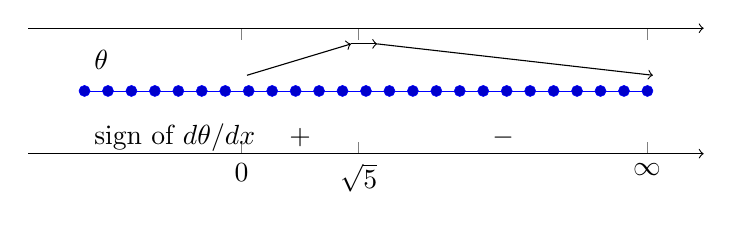
\begin{tikzpicture}
          \begin{axis}[axis y line=none, x axis line style={->}, 
          xtick={0,2.24,10-2.25}, xticklabels={$0$,$\sqrt{5}$,$\infty$},
          ymin=-2, ymax=2, height=1.25in, width=4in]
            \addplot+[domain=-3:10-2.24, very thin]{0};
            \draw (axis cs: -3, -1.5) node[right] {sign of 
                $d\theta/dx$};
            \draw (axis cs: -3, 1) node[right] {$\theta$};
            \draw (axis cs: 2.24/2, -1.5) node{$+$};
            \draw[->, xshift=2pt] (axis cs: 0, 0.5) -- (axis cs: 
              2.24-0.25, 1.5);
            \draw (axis cs: 5, -1.5) node{$-$};
            \draw[->, xshift=2pt] (axis cs: 2.24+0.25, 1.5) -- 
              (axis cs: 10-2.24, 0.5);
            \draw[->, xshift=2pt] (axis cs: 2.24-0.25, 1.5) --
              (axis cs: 2.24+0.25, 1.5);
          \end{axis}
        \end{tikzpicture}
    \end{center}
    Since $\diff{\theta}{x}$ is positive on $(0,\sqrt5$ and negative on
    $(\sqrt5,\infty)$, the maximum value of $\theta$ occurs when $x=5$.
    Therefore the tourist should stand \fbox{$\sqrt5$ feet} away from 
    the statue.
    \end{solution}


\spaceonly{\probonly{\newpage}}
  \item
    A block is attached to a spring; to describe the block's position, we
    use the variable $x$, as shown in the diagram.  If the block is at
    rest, it sits at the position $x = 0$.
    \begin{center}
      
\includegraphics[height=1in]{images/spring-diagram}
    \end{center}
    If the block is pushed/pulled, then it will oscillate horizontally.
    Suppose that it is oscillating with position at time $t$ given by
    \[ x(t) = \sqrt{3} \cos 3t + \sin 3t,\] where $x(t)$ is measured in cm
    and $t$ is measured in seconds.

    \begin{enumerate}

    \item
      \begin{problem}[\vfill]
        Find the velocity and acceleration of the mass at time $t$.
      \end{problem}

      \begin{solution}
        Since $v(t)=x'(t)$ and $a(t)=v'(t)=x''(t)$,
      
        \fbox{$v(t) = -3\sqrt{3} \sin(3t) + 3 \cos(3t)$} and 
        \fbox{$a(t) = -9\sqrt{3}\cos(3t) - 9\sin(3t)$.} 
      \end{solution}

      \note{If it comes up, you might want to point out that the acceleration is always in the direction opposite to the block's position relative to $0$. Students who are interested in physics might enjoy thinking about why that is.}

    \item
      \begin{problem}[\vfill]
        When does the mass pass through the equilibrium position ($x=0$) for
        the first time after $t = 0$?
      \end{problem}

      \begin{solution}

        We want to find the first value of $t$ greater than zero such that
        \[
          x(t) = \sqrt{3}\cos 3t + \sin 3t = 0.
        \]
        We can isolate $x$ on one side:
        \begin{align*}
          \sqrt{3}\cos 3t &= -\sin 3t \\
          -\sqrt{3} &= \tan 3t
        \end{align*}
        and solve the resulting equation. Let's substitute $u=3t$. Using
        the unit circle, we can determine that the
        first solution of $\tan u = -\sqrt{3}$ where $u$ is greater
        than zero is $u = \frac{2 \pi}{3}$. Switching back to $t$ gives us
        \fbox{$t=\frac{2\pi}{9}$.}
      \end{solution}

    \item
      \begin{problem}[\vfill]
        How far from its equilibrium position can the mass travel?
      \end{problem}

      \begin{solution}
        We want to find the maximum or minimum value of $x(t)$, whichever
        is larger in magnitude. First, we note that the period of $x(t)$
        is $\frac{2\pi}{3}$, since both $\cos 3t$ and $\sin 3t$ will repeat
        after $\frac{2\pi}{3}$. This means that we can restrict our
        attention to the interval $[0,\frac{2\pi}{3}]$. 

        Let's find the critical points. First, our endpoints are
        $t=0$ and $\frac{2\pi}{3}$. Next, we can set $x'(t)=0$:
        \begin{align*}
            x'(t) = -3\sqrt3 \sin 3t + 3 \cos 3t &= 0 \\
            3 \cos t 3t &= 3\sqrt3 \sin 3t \\
            \frac{1}{\sqrt3} = \tan 3t
        \end{align*}
        Let's substitute $u=3t$. In the interval $[0,2\pi]$, $\tan u =
        \frac{1}{\sqrt{3}}$ at $u=\frac{\pi}{6}$ and $\frac{7\pi}{6}$.
        Changing back to $t$ gives us $t=\frac{\pi}{18}$ and
        $\frac{7\pi}{18}$.

        By comparing the values of $x(t)$ at all critical points, we
        can determine that the maximum value of $2$ is attained at
        $t=\frac{\pi}{18}$ and the minimum value of $-2$ is attained at
        $t=\frac{7\pi}{18}$. Therefore the farthest the mass can travel
        is \fbox{2 cm} away from the equilibrium position.
      \end{solution}

    \item
      \begin{problem}[\vfill]
        What is the greatest speed the mass ever attains?
      \end{problem}

      \begin{solution}
        Speed is $|v(t)|$, so we want to find the most extreme
        value of $v(t)$,  which could be either the maximum or 
        the minimum value. Again, we can restrict our attention to
        the interval $[0,\frac{2\pi}{3}]$.

        We have critical points at the endpoints, $t=0$ and 
        $\frac{2\pi}{3}$. If we set $v'(t)=0$,
        \begin{align*}
        v'(t) = -9\sqrt3 \cos 3t - 9 \sin 3t &= 0 \\
        -9\sqrt 3 \cos 3t &= 9 \sin 3t \\
        -\sqrt3 = \tan 3t
        \end{align*}
        We solved this equation in part (b), and so we know that
        the first solution after $t=0$ is $t=\frac{2\pi}{9}$. 
        We can use the same steps to find the other solution:
        $t=\frac{5\pi}{9}$.

        By comparing the values of $v(t)$ at all critical points,
        we can determine that the maximum value of $6$ is achieved at
        $t= \frac{5\pi}{9}$, and the minimum value of $-6$ is achieved
        at $t=\frac{2\pi}{9}$. Thus, the greatest speed attained
        by the mass is $\SI{6}{\centi\meter\per\second}$.
      \end{solution}

    \item

      \begin{problem}[\vfill]
        According to this model, are the block and spring subject to
        friction?
      \end{problem}

      \begin{solution}
        No. If the block and spring were subject to friction, the mass
        would slow down over time, not oscillate periodically.
      \end{solution}

    \end{enumerate}

\pspace{\newpage}

 

\item  % (19.1.6 plus some)

Next class, we will return to the topic of limits, where we'll learn some powerful and important new limit techniques. To practice for this, evaluate the following limits. 
  
    \begin{enumerate}

    \item
      \begin{problem}[\vfill]
        $\displaystyle \lim_{x\to \infty} \sin x$
      \end{problem}

      \begin{solution}
        This limit does not exist since $\sin x$ oscillates repeatedly
        between $-1$ and $1$.
      \end{solution}

    \item
      \begin{problem}[\vfill]
        $\displaystyle \lim_{x\to \infty} \frac{\sin x}{x}$
      \end{problem}

      \begin{solution}
        This limit is \fbox{0}.  Since $\sin x$ oscillates between $-1$
        and $1$, $\frac{\sin x}{x}$ oscillates between $\frac{-1}{x}$ and
        $\frac{1}{x}$.  But both $\frac{-1}{x}$ and $\frac{1}{x}$ approach
        0 as $x \to \infty$, so $\frac{\sin x}{x}$ must also.  Here's an
        illustration, with the graph of $\frac{\sin x}{x}$ in black:
        \begin{center}
          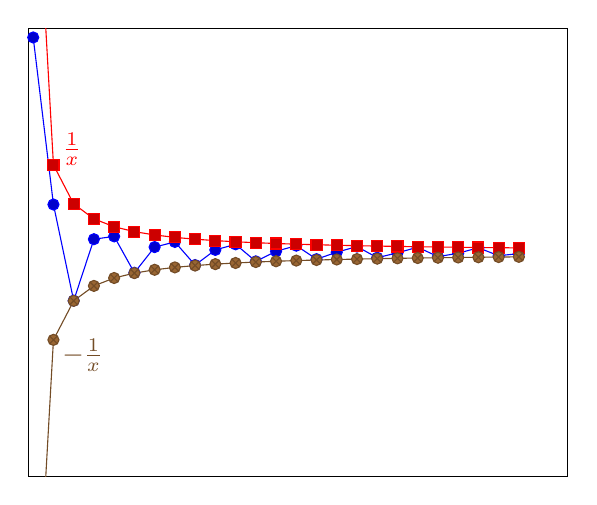
\begin{tikzpicture}
            \begin{axis}[xmin=0, xtick=\empty, ytick=\empty, ymin=-1, ymax=1]
              \addplot+[domain=0.5:50]{sin(deg(x))/x};
              \addplot+[domain=0.5:50]{1/x} node[pos=0.05,
              right]{$\frac{1}{x}$}; 
              \addplot+[domain=0.5:50]{-1/x} node[pos=0.05,
              right]{$-\frac{1}{x}$}; 
            \end{axis}
          \end{tikzpicture}
        \end{center}
      \end{solution}


    \item

      \note{This part and the next are just to remind them about dealing
        with potentially infinite limits.}

      \begin{problem}[\vfill]
        $\displaystyle \lim_{x\to 0^-} \frac{1}{ \sin x}$
      \end{problem}

      \begin{solution}
        As $x \to 0^-$, $\sin x \to 0$.  In this type of situation (that
        is, when we're looking at the limit of a fraction where the
        numerator approaches something nonzero and the denominator $\to
        0$), we should always think about the sign of the denominator.
        When $x$ is just a bit less than 0, $\sin x$ is always negative,
        so as $x \to 0^-$, $\sin x \to 0^-$.  Therefore, $\displaystyle
        \lim_{x\to 0^-} \frac{1}{ \sin x} = \boxed{-\infty}$ (when $x$ is
        a bit less than 0, $\sin x$ is a negative number which is very
        close to 0, so $\frac{1}{\sin x}$ is a very negative number).
      \end{solution}

    \item
      \begin{problem}[\vfill]
        $\displaystyle \lim_{x\to \frac{\pi}{2}} \frac{ \sin^2 x}{\cos x}
        $
      \end{problem}

      \begin{solution}
        As $x \to \frac{\pi}{2}$, $\sin^2 x \to \sin^2 \left(
          \frac{\pi}{2} \right) = 1$ and $\cos x \to \cos \frac{\pi}{2} =
        0$.  As in the previous part, this means we need to think about
        the sign of the denominator.  When $x$ is just a bit less than
        $\frac{\pi}{2}$, $\cos x$ is positive, so $\displaystyle \lim_{x
          \to \frac{\pi}{2}^-} \frac{ \sin^2 x}{\cos x} = \infty$.  When
        $x$ is just a bit bigger than $\frac{\pi}{2}$, $\cos x$ is
        negative, so $\displaystyle \lim_{x
          \to \frac{\pi}{2}^+} \frac{ \sin^2 x}{\cos x} = -\infty$.  Since
        the two one-sided limits don't agree, $\displaystyle \lim_{x\to
          \frac{\pi}{2}} \frac{ \sin^2 x}{\cos x}$ \fbox{does not exist}. 
      \end{solution}

    \end{enumerate}    
  

\end{enumerate}

\end{document}